% Title: gl2ps_renderer figure
% Creator: GL2PS 1.4.0, (C) 1999-2017 C. Geuzaine
% For: Octave
% CreationDate: Sun Dec  1 20:36:25 2019
\setlength{\unitlength}{1pt}
\begin{picture}(0,0)
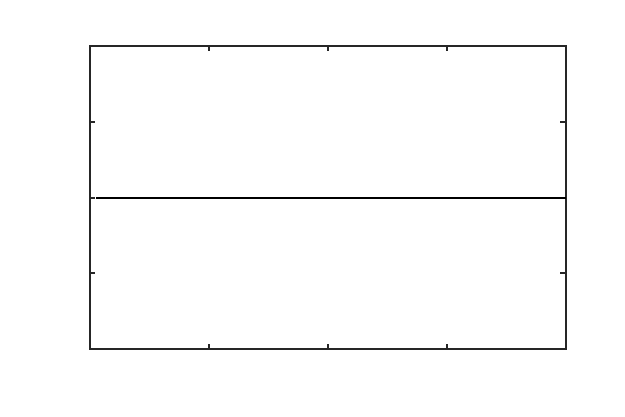
\includegraphics{img/phasePhiPPhi-inc}
\end{picture}%
\begin{picture}(300,200)(0,0)
\fontsize{10}{0}
\selectfont\put(42.9893,25){\makebox(0,0)[t]{\textcolor[rgb]{0.15,0.15,0.15}{{0}}}}
\fontsize{10}{0}
\selectfont\put(100.117,25){\makebox(0,0)[t]{\textcolor[rgb]{0.15,0.15,0.15}{{10}}}}
\fontsize{10}{0}
\selectfont\put(157.245,25){\makebox(0,0)[t]{\textcolor[rgb]{0.15,0.15,0.15}{{20}}}}
\fontsize{10}{0}
\selectfont\put(214.372,25){\makebox(0,0)[t]{\textcolor[rgb]{0.15,0.15,0.15}{{30}}}}
\fontsize{10}{0}
\selectfont\put(271.5,25){\makebox(0,0)[t]{\textcolor[rgb]{0.15,0.15,0.15}{{40}}}}
\fontsize{10}{0}
\selectfont\put(38,32.5246){\makebox(0,0)[r]{\textcolor[rgb]{0.15,0.15,0.15}{{0.9}}}}
\fontsize{10}{0}
\selectfont\put(38,68.8935){\makebox(0,0)[r]{\textcolor[rgb]{0.15,0.15,0.15}{{0.95}}}}
\fontsize{10}{0}
\selectfont\put(38,105.262){\makebox(0,0)[r]{\textcolor[rgb]{0.15,0.15,0.15}{{1}}}}
\fontsize{10}{0}
\selectfont\put(38,141.631){\makebox(0,0)[r]{\textcolor[rgb]{0.15,0.15,0.15}{{1.05}}}}
\fontsize{10}{0}
\selectfont\put(38,178){\makebox(0,0)[r]{\textcolor[rgb]{0.15,0.15,0.15}{{1.1}}}}
\fontsize{11}{0}
\selectfont\put(157.245,12){\makebox(0,0)[t]{\textcolor[rgb]{0.15,0.15,0.15}{{$\phi$}}}}
\fontsize{11}{0}
\selectfont\put(12,105.262){\rotatebox{90}{\makebox(0,0)[b]{\textcolor[rgb]{0.15,0.15,0.15}{{$p_{\phi}$}}}}}
\fontsize{11}{0}
\selectfont\put(157.245,188){\makebox(0,0)[b]{\textcolor[rgb]{0,0,0}{{Diagrama fase $\phi - p_\phi$}}}}
\end{picture}
